\documentclass[10pt]{scrartcl}
\usepackage[mdthm,colorsec,noauthor,noasy]{evan}
\usepackage{handout}
\newcommand{\aug}[2]{\left[\begin{array}{@{}#1@{}}#2\end{array}\right]}
\title{Math 54 --- Week 1}
\subtitle{Systems of linear equations; row reduction and echelon forms (Lay 1.1--1.2)}
\author{}\date{}\ihead{}
\begin{document}
\maketitle

\section{This week}

\subsection{Linear systems and their solution sets (Lay 1.1)}

\begin{qbox}
  Given several linear equations in several unknowns, how do we find every solution, and how can we tell quickly whether there is no solution, exactly one, or infinitely many?
\end{qbox}

\begin{definition*}
  A \vocab{linear equation} in the variables $x_1,\dots,x_n$ is an equation $a_1x_1+\dots+a_nx_n=b$ with numbers $a_1,\dots,a_n,b$. A \vocab{system of linear equations} (linear system) is a collection of such equations in the same variables. A \vocab{solution} is a list $(s_1,\dots,s_n)$ that makes every equation true when substituted. The \vocab{solution set} is the set of all solutions. Two systems are \vocab{equivalent} if they have the same solution set.
\end{definition*}
\begin{itemize}
  \ii $4x_1-5x_2+2=x_1$ is linear (rearrange to $3x_1-5x_2=-2$). $x_2=2\sqrt{x_1}-6$ and $x_1x_2+x_3=4$ are not: a variable appears under a root or multiplied by another variable.
  \ii A system is \vocab{consistent} if it has at least one solution, \vocab{inconsistent} if it has none.
\end{itemize}

\textbf{Three possibilities, seen with two equations in two unknowns.} Each equation is a line in the plane, and a solution is a point on both lines.
\begin{fig}
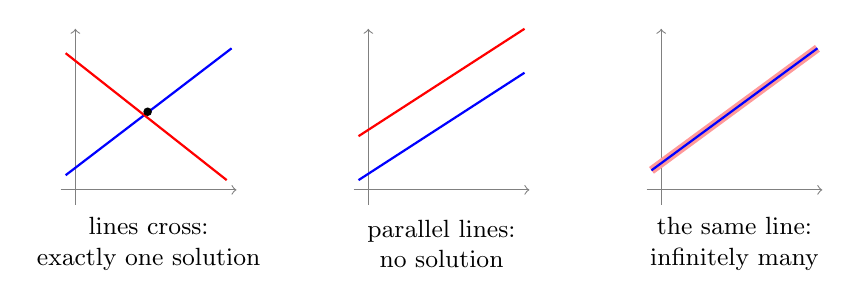
\begin{tikzpicture}[scale=0.62]
  \begin{scope}
    \draw[->,gray] (-0.3,0) -- (3.3,0); \draw[->,gray] (0,-0.3) -- (0,3.3);
    \draw[thick,blue] (-0.2,0.3) -- (3.2,2.9); \draw[thick,red] (-0.2,2.8) -- (3.1,0.2);
    \fill (1.48,1.6) circle (2.5pt);
    \node[font=\small,align=center] at (1.5,-1.1) {lines cross:\\exactly one solution};
  \end{scope}
  \begin{scope}[xshift=6cm]
    \draw[->,gray] (-0.3,0) -- (3.3,0); \draw[->,gray] (0,-0.3) -- (0,3.3);
    \draw[thick,blue] (-0.2,0.2) -- (3.2,2.4); \draw[thick,red] (-0.2,1.1) -- (3.2,3.3);
    \node[font=\small,align=center] at (1.5,-1.1) {parallel lines:\\no solution};
  \end{scope}
  \begin{scope}[xshift=12cm]
    \draw[->,gray] (-0.3,0) -- (3.3,0); \draw[->,gray] (0,-0.3) -- (0,3.3);
    \draw[line width=3pt,red!40] (-0.2,0.4) -- (3.2,2.9); \draw[thick,blue] (-0.2,0.4) -- (3.2,2.9);
    \node[font=\small,align=center] at (1.5,-1.1) {the same line:\\infinitely many};
  \end{scope}
\end{tikzpicture}
\figcap{Two lines meet in one point, in no point, or in every point of a common line. The existence and uniqueness theorem at the end of this handout shows that these are the only possibilities for every linear system, of any size.}
\end{fig}

\textbf{Matrix notation.} For the system
\[ \begin{aligned} x_1-2x_2+x_3&=0\\ 2x_2-8x_3&=8\\ 5x_1-5x_3&=10\end{aligned}
\qquad\text{coefficient matrix }
\begin{bmatrix}1&-2&1\\0&2&-8\\5&0&-5\end{bmatrix},\qquad
\text{augmented matrix }\aug{rrr|r}{1&-2&1&0\\0&2&-8&8\\5&0&-5&10}. \]
The \vocab{coefficient matrix} holds the coefficients of the variables; the \vocab{augmented matrix} adds the right-hand sides as a last column.
An $m\times n$ matrix has $m$ rows and $n$ columns. A missing variable has coefficient $0$.

\subsection{Elementary row operations}
\begin{definition*}
  The \vocab{elementary row operations} on a matrix are:
  \begin{enumerate}[(1)]
    \ii \textbf{Replacement}: replace a row by itself plus a multiple of another row.
    \ii \textbf{Interchange}: swap two rows.
    \ii \textbf{Scaling}: multiply all entries of a row by a \emph{nonzero} constant.
  \end{enumerate}
  Two matrices are \vocab{row equivalent} if one can be turned into the other by a sequence of elementary row operations.
\end{definition*}

\begin{theorem*}[Row operations do not change the solution set]
  If the augmented matrices of two linear systems are row equivalent, the two systems have the same solution set.
\end{theorem*}
\begin{ideabox}
Each row is an equation. A row operation builds new equations from old ones by adding, swapping or rescaling, so anything that satisfied the old equations satisfies the new ones: no solution is lost. Could a solution be \emph{gained}? Only if the operation threw away information. It does not, because every row operation can be undone by another row operation, and the undoing step also loses no solution. So solutions can be neither lost nor gained.
\end{ideabox}
\begin{proof}
  \begin{steps}
    \ii \emph{Each operation keeps every solution.} Let $(s_1,\dots,s_n)$ satisfy all the equations. Interchange and scaling (by $c\ne0$) produce equations that are the old ones in a different order or multiplied by $c$, so they still hold. For replacement, row $i$ becomes (row $i$) $+\,c\cdot$(row $j$); substituting gives (value of row $i$'s left side) $+\,c\cdot$(value of row $j$'s left side) $=b_i+cb_j$, which is the new right side.
    \ii \emph{Each operation can be reversed by another row operation.} Undo a replacement by subtracting the same multiple: (row $i$) $-\,c\cdot$(row $j$). Undo an interchange by swapping again. Undo scaling by $c$ by scaling by $1/c$; this is why scaling by $0$ is not allowed.
    \ii If the new system had a solution that the old one lacked, apply the reversing operations: by step 1 that solution would satisfy the old system. So the solution sets are equal. For a sequence of operations, apply this to each step.
  \end{steps}
\end{proof}

\textbf{Worked example: solving by elimination.}
\[ \aug{rrr|r}{1&2&-1&3\\2&5&1&14\\-1&1&4&9}
\xrightarrow[R_3+R_1]{R_2-2R_1}
\aug{rrr|r}{1&2&-1&3\\0&1&3&8\\0&3&3&12}
\xrightarrow{R_3-3R_2}
\aug{rrr|r}{1&2&-1&3\\0&1&3&8\\0&0&-6&-12} \]
\begin{steps}
  \ii The aim is triangular form: $x_1$ only in the first equation, $x_2$ not below the second, and so on. Use the first row to clear the first column below it, then the second row to clear the second column below it.
  \ii The last row says $-6x_3=-12$, so $x_3=2$. Back-substitute: $x_2=8-3x_3=2$, then $x_1=3-2x_2+x_3=1$.
  \ii Check in the original equations: $1+4-2=3$; $2+10+2=14$; $-1+2+8=9$.
\end{steps}

\textbf{Two fundamental questions} about any linear system: (1) \emph{Existence}: is it consistent? (2) \emph{Uniqueness}: if a solution exists, is it the only one? Both are answered by the echelon form below, without finding the solutions.

\subsection{Echelon forms (Lay 1.2)}
\begin{qbox}
  Elimination can be done in many orders. Is there a standard final shape that makes the solution set readable at a glance?
\end{qbox}
\begin{definition*}
  The \vocab{leading entry} of a row is its leftmost nonzero entry. A matrix is in \vocab{echelon form} if:
  \begin{enumerate}[(1)]
    \ii all nonzero rows are above any rows of all zeros;
    \ii each leading entry is in a column to the right of the leading entry of the row above it;
    \ii all entries in a column below a leading entry are zero.
  \end{enumerate}
  It is in \vocab{reduced echelon form} (RREF) if in addition:
  \begin{enumerate}[(1),start=4]
    \ii the leading entry in each nonzero row is $1$;
    \ii each leading $1$ is the only nonzero entry in its column.
  \end{enumerate}
\end{definition*}
\[ \text{echelon: }\begin{bmatrix}\blacksquare&*&*&*\\0&\blacksquare&*&*\\0&0&0&\blacksquare\\0&0&0&0\end{bmatrix}
\qquad\text{reduced echelon: }\begin{bmatrix}1&0&*&0\\0&1&*&0\\0&0&0&1\\0&0&0&0\end{bmatrix}
\qquad(\blacksquare\ne0,\ *\text{ any number}) \]

\begin{theorem*}[Uniqueness of the reduced echelon form]
  Each matrix is row equivalent to one and only one reduced echelon matrix.
\end{theorem*}
The proof is in Lay, Appendix A. An echelon form is \emph{not} unique (scaling a row changes it), but the RREF is. So the positions of the leading entries are the same in every echelon form of a matrix, and they get a name:
\begin{definition*}
  A \vocab{pivot position} of $A$ is a position that holds a leading $1$ in the RREF of $A$. A \vocab{pivot column} is a column containing a pivot position. A \vocab{pivot} is a nonzero number in a pivot position, used to create zeros.
\end{definition*}

\method{The row reduction algorithm.}
\begin{steps}
  \ii \emph{Forward phase.} Take the leftmost nonzero column; it is a pivot column, and its pivot position is at the top.
  \ii Choose a nonzero entry in that column as pivot, and interchange rows to move it to the top if needed.
  \ii Use replacement operations to create zeros in every position below the pivot.
  \ii Cover the row with the pivot (and all rows above it). Repeat steps 1--3 on the rows that remain, until none are left. The matrix is now in echelon form.
  \ii \emph{Backward phase.} Starting with the rightmost pivot and working up and to the left, create zeros above each pivot; scale each pivot row so the pivot is $1$. The matrix is now in RREF.
\end{steps}
\textbf{Why the order matters.} In the forward phase, once a row has been used as a pivot row and covered, later steps never touch it, and the zeros already created stay zero, because later replacements only add multiples of rows that are zero in those columns. In the backward phase, working from the right keeps the zeros to the left.

\subsection{Solutions of linear systems}
Take an augmented matrix to reduced echelon form and read it back as equations.
\begin{definition*}
  The variables corresponding to pivot columns of the coefficient matrix are \vocab{basic variables}. The others are \vocab{free variables}.
\end{definition*}
\textbf{Worked example: free variables.}
\[ \aug{rrrr|r}{1&3&0&-2&1\\2&6&1&-1&5\\-1&-3&1&5&2}
\xrightarrow[R_3+R_1]{R_2-2R_1}
\aug{rrrr|r}{1&3&0&-2&1\\0&0&1&3&3\\0&0&1&3&3}
\xrightarrow{R_3-R_2}
\aug{rrrr|r}{1&3&0&-2&1\\0&0&1&3&3\\0&0&0&0&0} \]
\begin{steps}
  \ii This is already reduced echelon form. Pivot columns: 1 and 3. Basic variables $x_1,x_3$; free variables $x_2,x_4$.
  \ii Each nonzero row has exactly one basic variable, so solve each row for its basic variable: $x_1=1-3x_2+2x_4$ and $x_3=3-3x_4$.
  \ii \textbf{Parametric description of the solution set:}
  \[ x_1=1-3x_2+2x_4,\qquad x_2\text{ is free},\qquad x_3=3-3x_4,\qquad x_4\text{ is free}. \]
  Every choice of $x_2,x_4$ gives a solution, and every solution arises this way. For example $x_2=x_4=0$ gives $(1,0,3,0)$.
\end{steps}
\textbf{Worked example: an inconsistent system.}
\[ \aug{rrr|r}{1&2&3&1\\2&5&4&2\\3&7&7&4}
\xrightarrow[R_3-3R_1]{R_2-2R_1}
\aug{rrr|r}{1&2&3&1\\0&1&-2&0\\0&1&-2&1}
\xrightarrow{R_3-R_2}
\aug{rrr|r}{1&2&3&1\\0&1&-2&0\\0&0&0&1} \]
The last row is the equation $0x_1+0x_2+0x_3=1$, which no numbers satisfy. The system is inconsistent; no further work is needed.

\begin{theorem*}[Existence and uniqueness]
  A linear system is consistent if and only if the rightmost column of the augmented matrix is \emph{not} a pivot column, that is, if and only if an echelon form of the augmented matrix has no row of the form $[\,0\ \cdots\ 0\ \ b\,]$ with $b\ne0$. If the system is consistent, then its solution set contains either exactly one solution (when there are no free variables) or infinitely many solutions (when there is at least one free variable).
\end{theorem*}
\begin{ideabox}
Read the echelon form as equations. A row $[\,0\ \cdots\ 0\ \ b\,]$ is the equation $0=b$. If $b\ne0$ it is false for every choice of the variables, which is the only way a system in echelon form can fail. Any other nonzero row has a leading entry in a variable column, so it can be solved for that basic variable once the later variables are known. Back-substitution then always succeeds, and the free variables are never constrained: each value of them gives one solution. So there is one solution if nothing is free, and one for each choice of the free variables (infinitely many) otherwise.
\end{ideabox}
\begin{proof}
  \begin{steps}
    \ii By the row operation theorem, the system has the same solutions as the system of its reduced echelon form, so we may read that form.
    \ii \emph{Rightmost column is a pivot column.} Then some row is $[\,0\ \cdots\ 0\ \ 1\,]$, the equation $0=1$. No solution.
    \ii \emph{Rightmost column is not a pivot column.} Then each nonzero row has its leading $1$ in the column of a basic variable, and that basic variable appears in no other row (condition (5) of RREF). So that row expresses the basic variable as a number minus a combination of free variables. Choosing any values for the free variables and computing the basic variables this way satisfies every equation. So the system is consistent.
    \ii If there are no free variables, step 3 gives each variable one value: exactly one solution. If there is a free variable, different values of it give different solutions: infinitely many.
  \end{steps}
\end{proof}
\method{Using row reduction to solve a linear system.}
\begin{steps}
  \ii Write the augmented matrix.
  \ii Row reduce to echelon form. If there is a row $[\,0\ \cdots\ 0\ \ b\,]$ with $b\ne0$, stop: no solution.
  \ii Otherwise continue to reduced echelon form.
  \ii Write each nonzero row as an equation and solve it for its basic variable in terms of the free variables.
  \ii State the solution parametrically, naming the free variables as free.
\end{steps}

\begin{shortcuts}
  \ii \textbf{Existence and uniqueness need only an echelon form}, not the RREF: look for a row $[\,0\cdots0\ b\,]$, $b\ne0$, and count pivots among the variable columns.
  \ii \textbf{Counting}: number of free variables $=$ (number of variables) $-$ (number of pivot columns of the coefficient matrix).
  \ii \textbf{More variables than equations}: there are at most as many pivots as rows, so a consistent system with more unknowns than equations always has a free variable, hence infinitely many solutions.
  \ii \textbf{Parameter questions} (``for which $h,k$ is the system consistent?''): row reduce with the letters in place; the answer is decided by the entries that end up in the last row. Watch for a pivot that could be zero, such as $8-4h$: split into the cases $h=2$ and $h\ne2$.
  \ii \textbf{Check} a solution by substituting it into the \emph{original} equations; this catches arithmetic slips at once.
  \ii \textbf{Avoid fractions} early: swap a row with a leading $1$ to the top, or scale at the end.
\end{shortcuts}
\begin{trapbox}
  \ii Scaling by $0$ is not a row operation (it cannot be undone).
  \ii Two operations in one step are safe only if neither uses a row the other changes. Doing $R_2\to R_2-R_1$ and $R_1\to R_1-R_2$ at the same time is not a sequence of row operations, and it can lose solutions.
  \ii A zero row $[\,0\ \cdots\ 0\ \ 0\,]$ is harmless; it does not by itself mean infinitely many solutions. Count free variables.
  \ii In the parametric description, each basic variable must be written in terms of free variables only. ``$x_3=1+x_2$'' when $x_2$ is basic does not describe the solution set.
  \ii An echelon form is not unique; the pivot positions are.
  \ii Pivot positions are those of the coefficient matrix when you count free variables; the augmented column is not a variable.
\end{trapbox}

\section{Homework this week}
HW1, Section 1.1: 1, 8, 9, 13, 17, 21, 25, 26, 27, 32, 34. Section 1.2: 1, 3, 11, 13, 15 (or 17), 19, 23, 25, 31, 32. (Sections 1.3--1.4 of HW1 are in the Week 2 handout.)

\section{Problem set}
\begin{prob}\textbf{P1.}\ Solve by row reduction and check your answer:
$x_1+x_2+2x_3=9,\quad 2x_1+4x_2-3x_3=1,\quad 3x_1+6x_2-5x_3=0.$
\end{prob}
\begin{prob}\textbf{P2.}\ For which $h$ is the system with augmented matrix $\aug{rr|r}{1&-3&h\\-2&6&-5}$ consistent?
\end{prob}
\begin{prob}\textbf{P3.}\ For the system $x_1+hx_2=2$, $4x_1+8x_2=k$, find all $h,k$ for which it has (a) no solution, (b) exactly one solution, (c) infinitely many solutions.
\end{prob}
\begin{prob}\textbf{P4.}\ Find the reduced echelon form and the parametric description of the solution set of the system with augmented matrix
$\aug{rrrrr|r}{1&-2&-1&3&0&-2\\0&0&1&-4&2&5\\2&-4&0&-2&2&1}.$
\end{prob}
\begin{prob}\textbf{P5.}\ True or false, with a reason. (a) A system of 3 equations in 4 unknowns can have exactly one solution. (b) If an echelon form of an augmented matrix has a row of zeros, the system has infinitely many solutions. (c) If the coefficient matrix of a system of 4 equations in 4 unknowns has a pivot in every column, the system has exactly one solution for every right-hand side.
\end{prob}
\begin{prob}\textbf{P6.}\ Find the polynomial $p(t)=a_0+a_1t+a_2t^2$ whose graph passes through $(1,4)$, $(2,9)$, $(3,18)$, by setting up and solving a linear system for $a_0,a_1,a_2$.
\end{prob}
\begin{prob}\textbf{P7.}\ Is the system $x+2y=5$, $3x-y=1$, $2x+3y=8$, $x+y=3$ consistent? If so, solve it.
\end{prob}

\end{document}
